\documentclass[english]{uzhpub}
\usepackage[T1]{fontenc}
\usepackage[latin9]{inputenc}
\usepackage{url}
\usepackage{hyperref}
\usepackage{epstopdf}

\hypersetup{
    colorlinks=true,
    linkcolor=black,
    filecolor=black,      
    urlcolor=black,
    citecolor=black
}

\begin{document}

%% Titelei
\title{The Import Content of Exports is Higher than the Leontief Inverse Suggests}

%\subtitle{}

\author{Luzius Meisser, luzius@meissereconomics.com}

\date{2016-04-19}

\maketitle

\emph{The Leontief inverse is the most popular tool to calculate the import reuse of exports from given input-output tables. However, because it implicitely assumes proportional use of inputs, it yields wrong results when applying it to aggregate sector data when the import intensities and export intensities of sectors beyond the resolution of the data are correlated, which usually is the case. Using data from the World Input-Output Database (WIOD), the Leontief inverse suggests a global import reuse of only 17\%  when based on one single aggregate sector per country, but results in much higher 24\% when based on all the 35 distinct sectors available in WIOD. Considering the plausible bounds and simulating further disaggregation beyond the resolution of the database under the assumption of self-similarity, I guess the true import content of exports to be even higher, namely around XX\% at average.}

\section{Introduction}
Import reuse, sometimes also called the import content of exports, is a basic metric that is typically derived from input-output tables and often serves as an intermediate step for more elaborate calculations, for example as a contributing factor when estimating exchange-rate pass-through. It measures the extent to which exports consist of previous imports. Its usual method of calculation is to derive the composition of exports by applying the Leontief inverse to the input-output table of the exporting country. \ref{OECD} More accurate results are achieved when basing the calculation on a worldwide input-output table such as WIOD, as this allows to account for circular flows of goods between country. \ref{Auer}

The subtle problem with this traditional approach is that the Leontief inverse implicitely assumes proportional use of inputs. In practice, however, firms that import much also tend to export much. \ref{Amiti} When aggregating such firms together with firms that have low import intensity, information about the actual use of specific imports gets lost and the import reuse as calculated by the Leontief inverse decreases. Thus, when the import intensity and the export intensity of sectors beyond the resolution of the data at hand are correlated, the Leontief inverse systematically underestimates import reuse.

After illustrating how strongly the reported import reuse depends on the resolution of the data, I construct a simple heuristic to artificially increase the resolution, thereby allowing to better estimate the true import reuse under the assumption of self-similarity between sectors at different resolutions. The source code of the used computer program is provided in a public repository\footnote{\href{https://github.com/kronrod/importreuse}{github.com/kronrod/importreuse}, with more detailed instructions in the repository itself.}, allowing anyone skilled in the art to reproduce these results within minutes and to calculate import reuse more accurately on their own datasets.

Subsequent section \ref{sec:data} describes the used data. It is followed by a detailed description of ...


\section{Data}
\label{sec:data}
\subsection{WIOD}
Using WIOD data from 2011.\\
Data coverage\\
Summary statistics (number obs, means, variances)\\
\subsection{Graph View}
\label{sec:graphview}
Usually, economists treat input-output tables as matrices. An equally valid and in this case more insightful view is to treat the input-output table as a weighted directed graph. Every square matrix can be represented as a weighted directed graph and a weighted directed graph can converted into a square matrix as long as there is at most one edge in each direction between each pair of nodes. In the graph representation of input-output tables, each node represents a sector in a country and named accordingly. Each weighted edge $e=(a, b, w)$ represents a flow from node $a$ to node $b$ of volume or weight $w$, as illustrated in figure X. Flows from a node to itself are allowed.

When merging two nodes $a$ and $b$ of a graph into a new node $c$, the nodes $a$ and $b$ are replaced by $c$ in all edges and then all edges that connect the same nodes in the same direction aggregated into a single new edge whose weight is the sum of the old weights. This is equivalent to removing column $i$ and adding it to column $j$ in the matrix view, and then also removing row $i$ and adding it to row $j$, with $i$ and $j$ being the indices of the two sectors represented by nodes $a$ and $b$. When doing so, the indices of other sectors may change, making it less convenient to track a specific sector in the matrix view than in the graph view, where the names of unaffected nodes stay the same when others are merged.

For simplicity, I merge each country's consumption types, capital formation, and inventory changes into one special node "consumption and capital accumulation" that is not counted as a sector. I.e., when later reducing the number of sectors per country to one, there will be two nodes left per country, one actual sector and the consumption node. Furthermore, I ignore negative flows into the consumption node\footnote{This can happen when capital is reduced or inventories decrease.} as they are negligible and not having negative edge weights is a prerequisite for some graph operations. All other flows in WIOD are zero or positive.

\section{Empirical Part}

\subsection{Plausible Bounds}
Illustration of the possible extremes using a simple graphic. Description of how the possible bounds are calculated, i.e. the import reuse under the assumption that imports are reexported first in each sector, and then the rest used domestically (if anything left).

\subsection{Varying the Sector Resolution}
When applying the Leontief inverse, the resulting import reuse depends on the resolution of the underlying data. This can be nicely demonstrated by starting with the full resolution provided by WIOD, namely 35 sectors, and then gradually reducing the resolution by merging sectors one by one, until only one large sector is left in each country. The resulting relation between number of sectors per country and calculated import reuse is depicted in figure \ref{fig:resolution}.

\begin{figure}
\centering
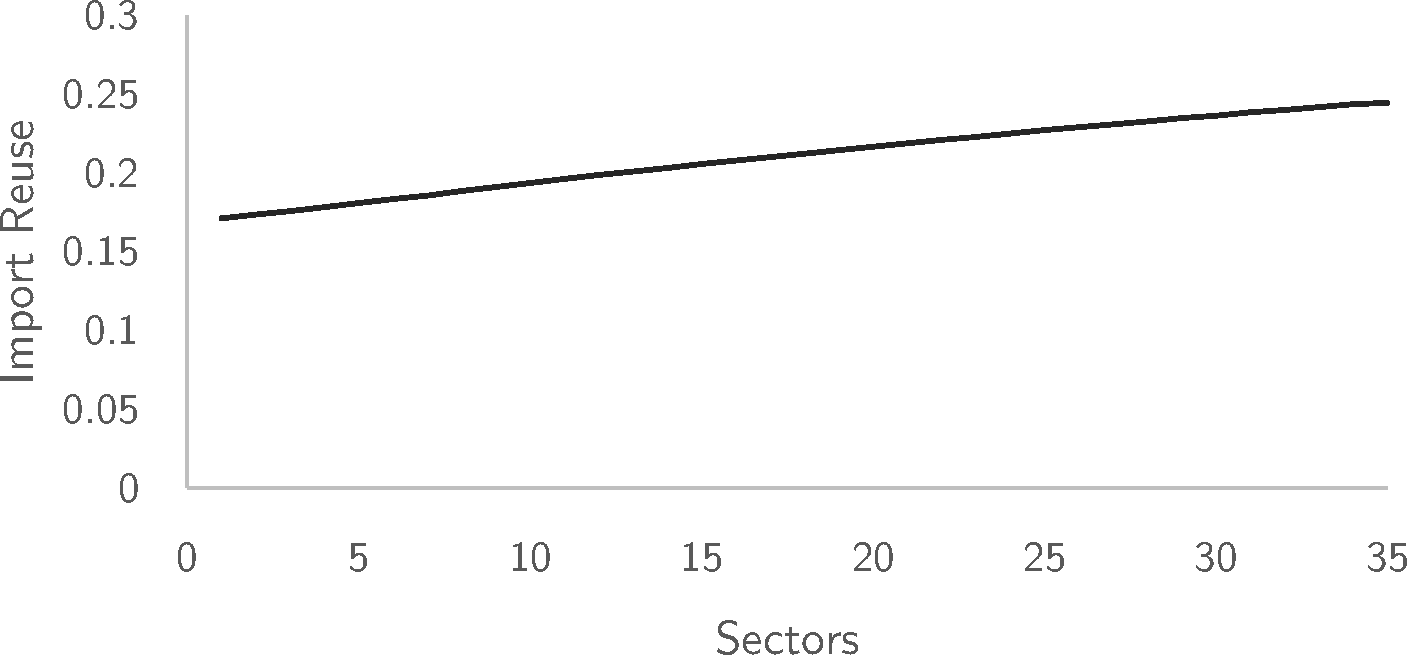
\includegraphics[scale=0.5]{../data/resolution}
\caption{The measured import reuse depends on the resolution of the underlying data. The plotted curve represents the average of 100 randomized runs. The standard deviation of each plotted point is less than $10^{-5}$, so the curve can be considered free from random variation.} \label{fig:resolution}
\end{figure}

The raw data for this figure has been generated with script \emph{Figure1Resolution}\footnote{\href{https://github.com/kronrod/importreuse/blob/master/src/com/meissereconomics/seminar/run/Figure1Resolution.java}{github.com/kronrod/importreuse/blob/master/src/com/meissereconomics/seminar/run/Figure1Resolution.java}}. It parses the 2005 world input-output table into a graph, calculates import reuse, and then reduces the number of sectors in each country by one. This is done by randomly selecting two sectors in each country and merging them as defined in section \ref{sec:graphview}. The reported import reuse is a global volume-weighted average of the import content of all exports. As the data is in graph form, import reuse is calculated by repeatedly updating the input composition of each node until all values have stabilized. This is equivalent to applying the Leontief inverse to the matrix view.

\subsection{Simulating Sector Splits}
Splitting a sector in two is the reverse of merging two sectors into one. Unfortunately, merging sectors is not a reversible operation as information gets lost when doing so. In order to simulate sector splits, a heuristic is needed to fill in the missing information, namely what share of the old weight should be assigned to the first new edge, and what share to the second. In the given context, it does not matter whether these simulated splits are realistic. All that matters is capturing the statistical properties that drive the changes in import reuse as the resolution is increased.

[Some comments on the statistial properties. Note that correlation of import intensity and export intensity is necessary, but not sufficient.

When splitting a node $c$ into two new nodes $a$ and $b$, all edges that contain $c$ are removed and replaced by two new edges that contain $a$ and $b$ in its place and that have positive weights whose sum equals the weight of the old edge.\footnote{In the special case of the edge $e=(c, c, w)$, four new edges $(a, a, w_1), (a, b, w_2), (a, b, w_3), (a, b, w - w_1 - w_2 - w_3)$ are created.} For each of the replaced edges, one must come up with a plausible way of splitting its weight, i.e. finding a plausible random variable $S \in [0,1]$  that says what share of the weight goes into the first edge. Figure \ref{fig:beta} plots a large number of realizations of $S$ in a histogram, suggesting that $S$ follows a beta-distribution with $\alpha=\beta\approx0.5$.

... more details description of approach, if it actually works. :) It is not implemented yet.


\subsection{Results}
Figure of how global import reuse grows as the number of sectors is increased.\\
Table of import content by country as estimated by Leontief inverse on 10 sectors, 35 sectors, and many simulated sectors.\\


\section{Discussion}
a.	Robustness vis-à-vis sub-samples / sub-period\\
b.	Correlation or causality?\\
c.	Limitations and further questions

Thought: Considering capital accumulation as consumption lowers the measured import reuse, as it can mask the foreign origin of domestic capital.

\section{Conclusion}

\end{document}
